% ------------------------------------------------------------------------------
% TYPO3 CMS 8.5 - What's New - Chapter "In-Depth Changes" (Spanish Version)
%
% @author	Michael Schams <schams.net>
% @license	Creative Commons BY-NC-SA 3.0
% @link		http://typo3.org/download/release-notes/whats-new/
% @language	English
% ------------------------------------------------------------------------------
% LTXE-CHAPTER-UID:		5ebcecbe-66abfa57-cf38bc00-aa637965
% LTXE-CHAPTER-NAME:	In-Depth Changes
% ------------------------------------------------------------------------------

\section{Cambios en Profundidad}
\begin{frame}[fragile]
	\frametitle{Cambios en Profundidad}

	\begin{center}\huge{Capítulo 3:}\end{center}
	\begin{center}\huge{\color{typo3darkgrey}\textbf{Cambios en Profundidad}}\end{center}

\end{frame}

% ------------------------------------------------------------------------------
% LTXE-SLIDE-START
% LTXE-SLIDE-UID:		18ffc2e2-e50d742a-879a153b-81aef243
% LTXE-SLIDE-ORIGIN:	bde270e6-ffef8544-ea472ed5-89ba8c3d English
% LTXE-SLIDE-TITLE:		#78581: FormEngine Data Providers
% ------------------------------------------------------------------------------

\begin{frame}[fragile]
	\frametitle{Cambios en Profundidad}
	\framesubtitle{Proveedores de Datos FormEngine}

	\begin{itemize}
		\item El proveedor de datos FormEngine \texttt{TcaFlexFetch} ha sido fusionado con \texttt{TcaFlexPrepare}
		\item Esto sólo afecta a instancias en el caso poco probable de que un proveedor de datos personalizado declaró una
			dependencia con \texttt{TcaFlexFetch}
	\end{itemize}

\end{frame}

% ------------------------------------------------------------------------------
% LTXE-SLIDE-START
% LTXE-SLIDE-UID:		881e1cec-a4fcec1b-6e93c162-bff70475
% LTXE-SLIDE-ORIGIN:	f0fb603c-54e9f255-03140395-b6b18103 English
% LTXE-SLIDE-TITLE:		#78384: Frontend ignores TCA in ext_tables.php
% ------------------------------------------------------------------------------
\begin{frame}[fragile]
	\frametitle{Cambios en Profundidad}
	\framesubtitle{TCA en \texttt{ext\_tables.php}}

	\begin{itemize}
		\item Peticiones frontend no se cargan más sobre \texttt{ext\_tables.php} en las peticiones
		\item Este cambio tiene un impacto sobre extensiones que configuran el TCA en \texttt{ext\_tables.php}\newline
			\small(que no está permitido de todos modos)\normalsize
		\item La Herramienta de Instalación proporciona un test "chequeo de TCA ext\_tables" para identificar tales extensiones
	\end{itemize}

	\begin{figure}
		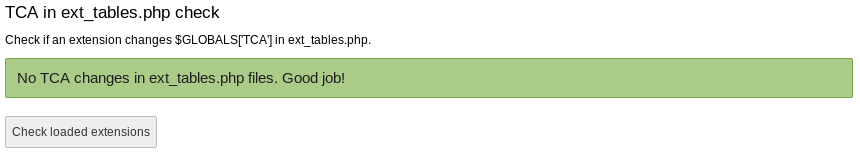
\includegraphics[width=0.95\linewidth]{InDepthChanges/78384-install-tool-tca-in-exttables-check.png}
	\end{figure}

\end{frame}
% ------------------------------------------------------------------------------
% LTXE-SLIDE-START
% LTXE-SLIDE-UID:		23ee3c3d-3a1e1a27-5ac629b6-6d50b4c5
% LTXE-SLIDE-ORIGIN:	bdcd2449-b679717b-9f23eb32-018953b4 English
% LTXE-SLIDE-TITLE:		#78191: Remove support for transForeignTable/transOrigPointerTable in TCA
% ------------------------------------------------------------------------------
\begin{frame}[fragile]
	\frametitle{Cambios en Profundidad}
	\framesubtitle{TCA en \texttt{ext\_tables.php}}

	\begin{itemize}
		\item Las tablas de base de datos que mantienen registros localizados y traducidos eran configurables en el TCA

			\begin{itemize}
				\item \texttt{\$TCA[<table\_name>]['ctrl']['transForeignTable']}\newline
					(usualmente apuntaba a la tabla: \texttt{pages\_language\_overlay})
				\item \texttt{\$TCA[<table\_name>]['ctrl']['transOrigPointerTable']}\newline
					(usualmente apuntaba a la tabla: \texttt{pages})
			\end{itemize}

		\item Esta configuración ha sido reemplazada con nombres de tabla codificados para prevenir
			el manejo especial y prepararse para una combinación de ambas tablas en el futuro

	\end{itemize}

\end{frame}

% ------------------------------------------------------------------------------
% LTXE-SLIDE-START
% LTXE-SLIDE-UID:		6a4615f1-895230b8-1db37e5b-8c85d531
% LTXE-SLIDE-ORIGIN:	ede02440-cafd3417-eb416f09-8e024ef2 English
% LTXE-SLIDE-TITLE:		#78383: Tables removed from defaultCategorizedTables
% ------------------------------------------------------------------------------
\begin{frame}[fragile]
	\frametitle{Cambios en Profundidad}
	\framesubtitle{Tablas eliminadas de \texttt{defaultCategorizedTables}}

	\begin{itemize}
		\item Las siguientes tablas han sido eliminadas de \texttt{defaultCategorizedTables}:

			\begin{itemize}
				\item \texttt{pages}
				\item \texttt{tt\_content}
				\item \texttt{sys\_file\_metadata}
			\end{itemize}

		\item Para estas tablas el núcleo API\newline
			\texttt{ExtensionManagementUtility::makeCategorizable()}\newline
			es ejecutado para definir una posición común del campo categorías

	\end{itemize}

\end{frame}


% ------------------------------------------------------------------------------
% LTXE-SLIDE-START
% LTXE-SLIDE-UID:		844b9db7-2f5f135e-8b7e0071-6fd4a8ac
% LTXE-SLIDE-ORIGIN:	dd31e5d5-ca09ae5e-eb87d926-0ffe8f0a English
% LTXE-SLIDE-TITLE:		Low-level parameters changes (1)
% ------------------------------------------------------------------------------
\begin{frame}[fragile]
	\frametitle{Cambios en Profundidad}
	\framesubtitle{Cambios de Parámetros de Bajo-Nivel (1)}

	% changes: #78417, #78439, #78520, #78552, #78577, #78623, #78627 and #78895

	\begin{itemize}
		\item Los comandos de bajo nivel listados abajo usan la Consola de Symfony ahora
		\item Nuevos comandos se comportan como los viejos, pero permitiendo usar ciertos parámetros

			\begin{itemize}
				\item \texttt{DeletedRecordsCommand}
				\item \texttt{CleanFlexFormsRecordsCommand}
				\item \texttt{OrphanRecordsCommand}
				\item \texttt{LostFilesCommand}
				\item \texttt{MissingFilesCommand}
				\item \texttt{MissingRelationsCommand}
				\item \texttt{DoubleFilesCommand}
				\item \texttt{RteImagesCommand}
			\end{itemize}

	\end{itemize}

\end{frame}



% ------------------------------------------------------------------------------
% LTXE-SLIDE-START
% LTXE-SLIDE-UID:		8e0ac428-16a282f4-de0e2d91-c2d8014f
% LTXE-SLIDE-ORIGIN:	3a9d25bb-d948368d-e2a92666-6170eaad English
% LTXE-SLIDE-TITLE:		Low-level parameters changes (2)
% ------------------------------------------------------------------------------
\begin{frame}[fragile]
	\frametitle{Cambios en Profundidad}
	\framesubtitle{Cambios de Parámetros de Bajo-Nivel (2)}

	% changes: #78417, #78439, #78520, #78552, #78577, #78623, #78627 and #78895

	\begin{itemize}
		\item Las clases PHP relacionadas han sido eliminadas\newline
			\smaller(p.e. \texttt{TYPO3\textbackslash
				CMS\textbackslash
				Lowlevel\textbackslash
				DeletedRecordsCommand})
			\normalsize

		\item Ejecutar el comando vía \texttt{cli\_dispatch} no funciona más\newline
			\smaller(p.e. \texttt{limpiador de bajo nivel typo3/cli\_dispatch eliminado})\normalsize
		\item Llamar a la clase PHP resulta en un error PHP fatal ahora

		\item Los comandos pueden ser ahora ejecutados vía CLI como sigue:\newline
			\smaller\texttt{/typo3/sysext/core/bin/typo3 cleanup:<command>}\normalsize\newline
			por ejemplo:\newline
			\smaller\texttt{/typo3/sysext/core/bin/typo3 cleanup:deletedrecords}\normalsize

	\end{itemize}

\end{frame}




% ------------------------------------------------------------------------------
% LTXE-SLIDE-START
% LTXE-SLIDE-UID:		b379b38d-cd3da3e4-96401a06-0a58d960
% LTXE-SLIDE-ORIGIN:	ec6817fd-c3364ffb-c74e9523-a18a3095 English
% LTXE-SLIDE-TITLE:		Re-factor FlexForm Data Structure Handling
% ------------------------------------------------------------------------------
\begin{frame}[fragile]
	\frametitle{Cambios en Profundidad}
	\framesubtitle{Re-factorizar Manejo de Estructura de Datos FlexForm}

	% https://forge.typo3.org/issues/78581
	% https://forge.typo3.org/issues/78616
	% https://forge.typo3.org/issues/78852
	% https://forge.typo3.org/issues/69715

	\begin{itemize}
		\item Con la deprecación de \texttt{BackendUtility::getFlexFormDS()} el hook
			\texttt{getFlexFormDSClass} no es llamado más

	\end{itemize}

\end{frame}





% ------------------------------------------------------------------------------
% LTXE-SLIDE-START
% LTXE-SLIDE-UID:		40f1ccbb-e9ee20be-b62fbab3-e340c9ec
% LTXE-SLIDE-ORIGIN:	b400c3b8-3e402480-cd7d6ff3-96cd93aa English
% LTXE-SLIDE-TITLE:		#76085: Add fluid debug information to admin panel
% ------------------------------------------------------------------------------
\begin{frame}[fragile]
	\frametitle{Cambios en Profundidad}
	\framesubtitle{Panel Admin}

	\begin{itemize}
		\item Panel Admin cuenta con un nuevo ajuste para depurar salida Fluid:\newline
			\textbf{Previsualizar -> Mostrar salida de depuración fluid}
		\item Si se habilita, los siguientes detalles se muestran en el frontend:

			\begin{itemize}
				\item ruta al fichero de template de un parcial
				\item nombre de una sección
			\end{itemize}

		\item Esta característica permite a los integradores fácilmente localizar el template correcto y la sección

	\end{itemize}

\end{frame}






% ------------------------------------------------------------------------------
% LTXE-SLIDE-START
% LTXE-SLIDE-UID:		fbed0415-acf84c32-aa39998b-2546a42c
% LTXE-SLIDE-ORIGIN:	60a2d39f-f04b8bf1-dc758912-607ed07e English
% LTXE-SLIDE-TITLE:		#52286: System Status Updates Report via email
% ------------------------------------------------------------------------------
\begin{frame}[fragile]
	\frametitle{Cambios en Profundidad}
	\framesubtitle{Actualizaciones de Estado del Sistema (Informes)}

	\begin{itemize}
		\item Los resultados de test en las "Actualizaciones de Estado del Sistema (informes)" pueden ser enviados vía email
		\item Una casilla ha sido añadida a la configuración de la tarea para:

			\begin{itemize}
				\item enviar un email si el sistema tiene advertencias o errores
				\item siempre generar un email
			\end{itemize}

		\item El valor por defecto es incluir advertencias y errores sólo

	\end{itemize}

\end{frame}







% ------------------------------------------------------------------------------
% LTXE-SLIDE-START
% LTXE-SLIDE-UID:		a0f72e71-277d72bc-42f22925-d2f42ca0
% LTXE-SLIDE-ORIGIN:	e4e2ead3-c07beb21-e8100580-d0e7c756 English
% LTXE-SLIDE-TITLE:		#58637: Purge language packs in language module
% ------------------------------------------------------------------------------
\begin{frame}[fragile]
	\frametitle{Cambios en Profundidad}
	\framesubtitle{Paquetes de Lenguaje}

	\begin{itemize}
		\item Desactivar los lenguajes en el módulo "Lenguajes" dejaba datos de lenguaje sobrantes
			en la carpeta \texttt{typo3conf/l10n/<locale>/}
		\item Un botón de "eliminado" ha sido añadido, que deshabilita el lenguaje y borra los
			datos en la carpeta
	\end{itemize}

\end{frame}








% ------------------------------------------------------------------------------
% LTXE-SLIDE-START
% LTXE-SLIDE-UID:		88ec32bf-7d9e6b76-f40cec1c-52cf33b9
% LTXE-SLIDE-ORIGIN:	08961fb3-00cbc9f4-964f8d01-6e59e782 English
% LTXE-SLIDE-TITLE:		#67909: Hook added to localize() function
% ------------------------------------------------------------------------------
\begin{frame}[fragile]
	\frametitle{Cambios en Profundidad}
	\framesubtitle{Hook en DataHandler \texttt{localize()}}

	% decrease font size for code listing
	\lstset{basicstyle=\tiny\ttfamily}

	\begin{itemize}
		\item Se ha añadido un nuevo hook para la función \texttt{localize()}
		\item Esto permite por ejemplo usar servicios de traducción externos o funciones de transliteración
			personalizadas que manejan varias transformaciones de contenido
	\end{itemize}

	\begin{itemize}
		\item Hook:\newline
			\smaller
				\texttt{\$GLOBALS['TYPO3\_CONF\_VARS']['SC\_OPTIONS']\newline
				\tabto{0.4cm}['t3lib/class.t3lib\_tcemain.php']['processTranslateToClass']}
			\normalsize

		\item Uso de ejemplo:

			\begin{lstlisting}
				class YourHookClass
				{
				  public function processTranslateTo_copyAction(&$content, $lang, $dataHandler)
				  {
				    // Do something with content (translate, transliterate etc.)
				  }
				}
			\end{lstlisting}
	\end{itemize}

\end{frame}









% ------------------------------------------------------------------------------
% LTXE-SLIDE-START
% LTXE-SLIDE-UID:		b41d8c6e-13fe8197-e4b97049-0e3c3c20
% LTXE-SLIDE-ORIGIN:	8b1a9661-d6fab90f-9c856224-ee663aa2 English
% LTXE-SLIDE-TITLE:		#77757: Re-check if an UpdateWizard should run
% ------------------------------------------------------------------------------
\begin{frame}[fragile]
	\frametitle{Cambios en Profundidad}
	\framesubtitle{Asistente de Actualización}

	\begin{columns}[T]
		\begin{column}{.5\textwidth}
			El Asistente de Actualización en la Herramienta de Instalación lista todas las tareas marcadas como \textit{completadas}.
			\newline\newline
			Casillas y un botón "Rechequear asistentes elegidos" permiten reiniciar las actualizaciones.
			El asistente testeará si la tarea necesita ser ejecutada otra vez.
		\end{column}
		\begin{column}{.5\textwidth}
			\begin{figure}\vspace*{-0.5cm}
				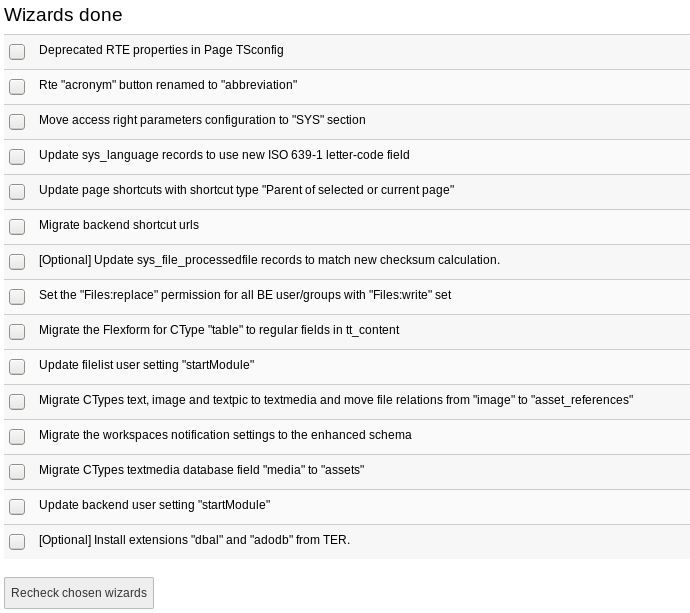
\includegraphics[width=0.8\linewidth]{InDepthChanges/77757-upgrade-wizard.png}
			\end{figure}
		\end{column}
	\end{columns}

\end{frame}









% ------------------------------------------------------------------------------
% LTXE-SLIDE-START
% LTXE-SLIDE-UID:		0405984f-22a9e22d-85079837-a3a3f928
% LTXE-SLIDE-ORIGIN:	94640f3d-0f632507-a2166719-5adc755e English
% LTXE-SLIDE-TITLE:		#78523: Suggest wizard provides option to define ordering of results
% ------------------------------------------------------------------------------
\begin{frame}[fragile]
	\frametitle{Cambios en Profundidad}
	\framesubtitle{Asistente de Sugerencias}

	% decrease font size for code listing
	\lstset{basicstyle=\tiny\ttfamily}

	\begin{itemize}
		\item El FormEngine ("TCEforms") permite configurar el orden de los resultados por el asistente de sugerencias
		\item La nueva opción es una definición de order-by estándar SQL:\newline
			\small\texttt{'orderBy' => 'field ASC/DESC'}\normalsize
		\item Configuración de ejemplo TCA:

			\begin{lstlisting}
				'config' => [
				  ...
				  'wizards' => [
				    'suggest' => [
				      'type' => 'suggest',
				      'default' => [
				        'searchWholePhrase' => true,
				        'addWhere' => ' AND tx_news_domain_model_news.uid != ###THIS_UID###',
				        'orderBy => 'datetime DESC',
				      ]
				    ],
				  ],
				]
			\end{lstlisting}

	\end{itemize}

\end{frame}











% ------------------------------------------------------------------------------
% LTXE-SLIDE-START
% LTXE-SLIDE-UID:		6952ed0a-e51b3e5d-e0634765-ccc6ed95
% LTXE-SLIDE-ORIGIN:	0907e5d3-a12751cb-23f49488-7a05a208 English
% LTXE-SLIDE-TITLE:		Miscellaneous
% ------------------------------------------------------------------------------
\begin{frame}[fragile]
	\frametitle{Cambios en Profundidad}
	\framesubtitle{Miscelánea (1)}

	% #78103: Add missing information status for addSystemMessage
	% #78575: Get enumeration constants
	% #75232: Spread TypeConverter priorities

	\begin{itemize}
		\item Toda la información del sistema añadida por \texttt{addSystemInformation()} tiene
			\texttt{InformationStatus::STATUS\_NOTICE} como el valor por defecto ahora
		\item Constantes de enumeración pueden ser recuperadas ahora fácilmente:

			\begin{itemize}
				\item \texttt{EnumerationClass::getName(\$value);}
				\item \texttt{EnumerationClass::getHumanReadableName(\$value);}
			\end{itemize}

		\item Prioridades del núcleo TypeConverters han cambiado de\newline
			\texttt{1}, \texttt{2}, \texttt{3},... a \texttt{10}, \texttt{20}, \texttt{30},...
			Al registrar TypeConverter(s) personalizados, asegúrese de que están usando las prioridades correctas.

	\end{itemize}

\end{frame}







% ------------------------------------------------------------------------------
% LTXE-SLIDE-START
% LTXE-SLIDE-UID:		6952ed0a-e51b3e5d-e0634765-ccc6ed95
% LTXE-SLIDE-ORIGIN:	0907e5d3-a12751cb-23f49488-7a05a208 English
% LTXE-SLIDE-TITLE:		Miscellaneous
% ------------------------------------------------------------------------------
\begin{frame}[fragile]
	\frametitle{Cambios en Profundidad}
	\framesubtitle{Miscelánea (2)}

	% #78103: Add missing information status for addSystemMessage
	% #78575: Get enumeration constants
	% #75232: Spread TypeConverter priorities

	\begin{itemize}
		\item \href{https://en.wikipedia.org/wiki/ISO_8601}{ISO-8601} es usado para pasar valores de fechas y horas
			entre el servidor y el cliente ahora. Compruebe si los tipos de renderizado FormEngine personalizados necesitan
			ser actualizados (\texttt{eval=date/datetime}).

	\end{itemize}

\end{frame}





% ------------------------------------------------------------------------------
